%!TEX root = base.tex

\chapter{Previous Work}

Modelling of Wi-Fi performance characteristics is an active field of research
and this chapter provides an introduction to the approach invented by Bianchi
and the subsequent efforts made by others, in particular Ekici and Felemban.

\section{Modelling IEEE 802.11}

There are two ways of to estimate performance of a network: by way of analytic
models or simulation. This thesis considers only analytic models.

Today, analytical models are used in peformance and capacity estimation and
optimization.

\section{The Bianchi Model}

In \cite{bianchi}, Bianchi presented a novel approach to modeling of IEEE
802.11 DCF performance using a Tagged-Node Markov Chain (TNMC), see Figure
\ref{fig:tnmc}. The key assumption is to envision a network of identical
nodes. Modelling the peformance of the network or of a single node are
equivalent, with the latter being much simpler. Thus only the performance of a
single node, the \emph{Tagged Node}, is modeled. 

The model only considers single-hop, fully connected networks (see Figure
\ref{fig:shfc}) under saturation, defined as nodes always wanting to transmit.
Of course, networks in the wild are not going to be single-hop, considering
the rising use of repeaters, and will most probably contain hidden nodes (not
fully connected).

Bianchi's model ignores several important behaviors of the DCF, in particular
retransmission limit and backoff counter freezing due to channel state. Figure
\ref{fig:tnmc} does not describe to the original Bianchi model, but can be
made similar with $P_f = 0$. Others have explored many ways to extend and
improve the Bianchi model, especially regarding these two behaviors. 

\begin{figure}
\center
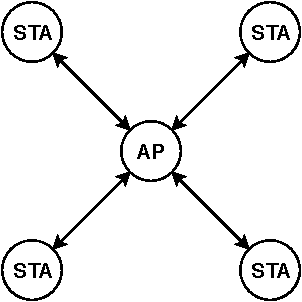
\includegraphics[width=0.15\textwidth]{images/shfc-network.pdf}
\caption{Single-hop fully-connected IEEE 802.11 network with 5 nodes: 1 access point (AP) and 4 stations (STA)}
\label{fig:shfc}
\end{figure}

\section{The Felemban-Ekici Model}

\begin{figure}
\center
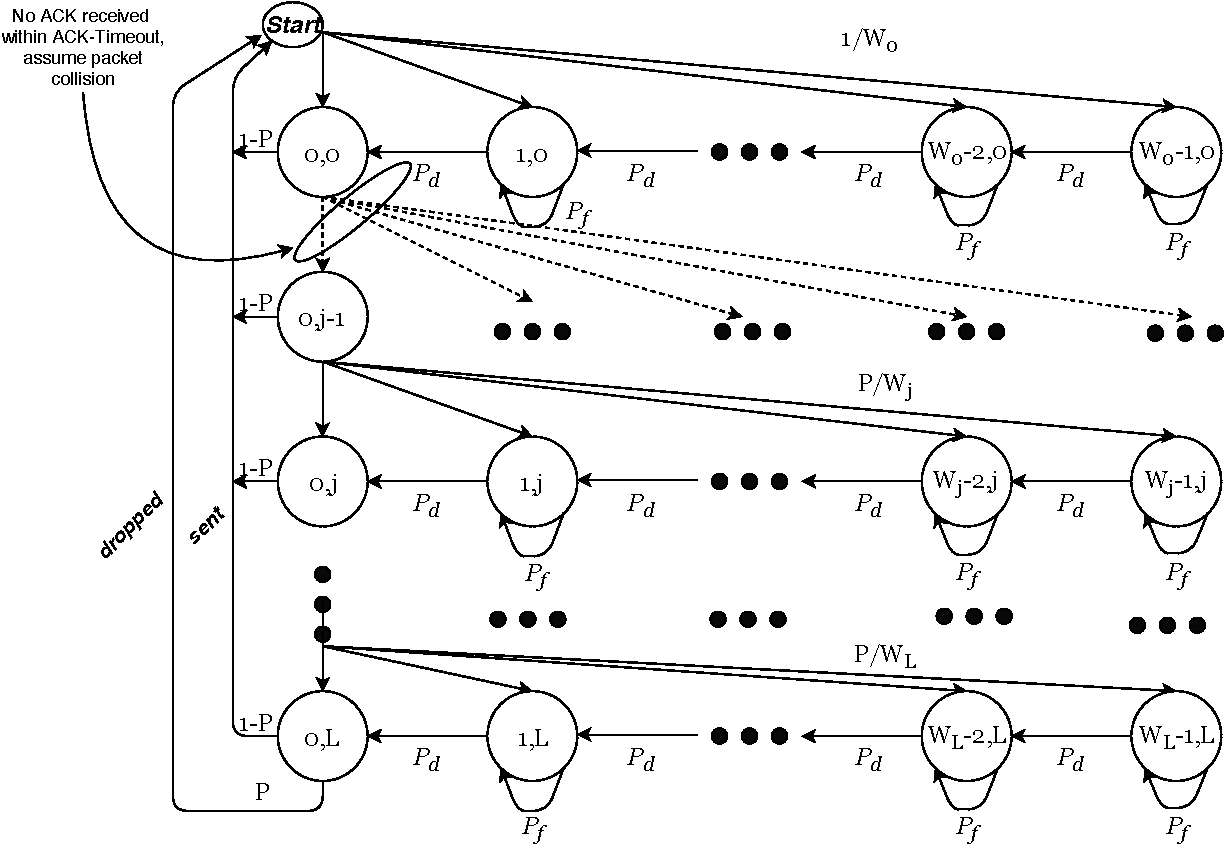
\includegraphics[width=1\textwidth]{images/tnmc-dcf.pdf}
\caption{Extended Tagged-Node Markov Chain (TNMC) model of the IEEE 802.11 DCF. $P$ is packet collision probability, $P_d$ is probability to decrease backoff counter, $P_f = 1 - P_d$, $W_j$ is contention window size at attempt $j$ and $L$ is the Short Retry Limit}
\label{fig:tnmc}
\end{figure}

In 2011, E. Felemban \& E. Ekici published an extended version of Bianchi's model, where they significantly improved the model's accuracy by introducing a more accurate behaviour of the entry into backoff and the backoff countdown procedure \cite{felemban}.

An overview of this TNMC model is presented in Figure \ref{fig:tnmc}. Readers
are refered to \cite{bianchi}, ... and x, for a more accurate representation
of their respective models.

Recall the DCF backoff behavior from \ref{fig:dcfgraph}, where the node waits
and only decrements the backoff counter if the channel was sensed idle. In
\cite{felemban}, the authors achieved a more accurate countdown probability
($P_d$) by introducing an additional markov chain to model the channel-sensing
process and estimating the probability of \emph{not} counting down, i.e.
probability of counter freeze ($P_f$), called Channel-Sense Markov Chain
(CSMC).

The counter freeze probability, $P_f$, is computed by finding the steady state
probabilities of the CSMC. Solving for the steady states is done by
fixed-point iteration—iterative computation until the difference between the
current and previous solution is less than some small value $\epsilon$.

While the model proposed by Ekici-Felemban models the DCF more closely and
accurately, several assumptions and constraints inherited from the markov
chain approximation makes the model a very interesting candidate for
real-world testing.

\subsection{The Unsaturated Model}

This approach, while performing better than others, yielded a simpler model
for the unsaturated case.